% ------ headers globales -------------
\documentclass[11pt, a4paper, twoside]{article}
\usepackage{header}
\usepackage{config}
% -------------------------------------
\begin{document}

%-- Carátula --
\clearpage{\pagestyle{empty}% **************************************************************************
%
%  Package 'caratula', version 0.3 (para componer caratulas de TPs del DC).
%
%  En caso de dudas, problemas o sugerencias sobre este package escribir a
%  Brian J. Cardiff (bcardif arroba gmail.com).
%  Nico Rosner (nrosner arroba dc.uba.ar).
%
% **************************************************************************

% ----- Informacion sobre el package para el sistema -----------------------

\NeedsTeXFormat{LaTeX2e}
\ProvidesPackage{caratula}[2005/08/09 v0.3 Para componer caratulas de TPs del DC]
\usepackage[pdftex]{graphicx}

% ----- Imprimir un mensajito al procesar un .tex que use este package -----

\typeout{Cargando package 'caratula' v0.3 (2005/08/09)}

% ----- Algunas variables --------------------------------------------------

\let\Materia\relax
\let\Submateria\relax
\let\Titulo\relax
\let\Subtitulo\relax
\let\Grupo\relax
\let\Fecha\relax
\let\Logoimagefile\relax
\let\Resumen\relax
\let\Tags\relax

% ----- Comandos para que el usuario defina las variables ------------------

\def\materia#1{\def\Materia{#1}}
\def\submateria#1{\def\Submateria{#1}}
\def\titulo#1{\def\Titulo{#1}}
\def\subtitulo#1{\def\Subtitulo{#1}}
\def\grupo#1{\def\Grupo{#1}}
\def\fecha#1{\def\Fecha{#1}}
\def\logoimagefile#1{\def\Logoimagefile{#1}}
\def\resumen#1{\def\Resumen{#1}}
\def\tags#1{\def\Tags{#1}}

% ----- Token list para los integrantes ------------------------------------

\newtoks\intlist\intlist={}

% ----- Comando para que el usuario agregue integrantes --------------------

\def\integrante#1#2#3{\intlist=\expandafter{\the\intlist
    \rule{0pt}{1.2em}#1&#2&\tt #3\\[0.2em]}}

% ----- Macro para generar la tabla de integrantes -------------------------

\def\tablaints{%
    \begin{tabular}[t]{| l @{\hspace{4ex}} c @{\hspace{4ex}} l|}
        \hline
        \multicolumn{1}{|c}{\rule{0pt}{1.2em} Integrante} & LU &  \multicolumn{1}{c|}{Correo electr\'onico} \\[0.2em]
        \hline \hline
        \the\intlist
        \hline
    \end{tabular}}

% ----- Codigo para manejo de errores --------------------------------------

\def\se{\let\ifsetuperror\iftrue}
\def\ifsetuperror{%
    \let\ifsetuperror\iffalse
    \ifx\Materia\relax\se\errhelp={Te olvidaste de proveer una \materia{}.}\fi
    \ifx\Titulo\relax\se\errhelp={Te olvidaste de proveer un \titulo{}.}\fi
    \edef\mlist{\the\intlist}\ifx\mlist\empty\se%
    \errhelp={Tenes que proveer al menos un \integrante{nombre}{lu}{email}.}\fi
    \expandafter\ifsetuperror}


% ----- \maketitletxt correspondiente a la versión v0.2 (texto) ---------

\def\maketitletxt{%
    \ifsetuperror\errmessage{Faltan datos de la caratula! Ingresar 'h' para mas informacion.}\fi
    \thispagestyle{empty}
    \begin{center}
    \vspace*{\stretch{2}}
    {\LARGE\textbf{\Materia}}\\[1em]
    \ifx\Submateria\relax\else{\Large \Submateria}\\[0.5em]\fi
    \par\vspace{\stretch{1}}
    {\large Departamento de Computaci\'on}\\[0.5em]
    {\large Facultad de Ciencias Exactas y Naturales}\\[0.5em]
    {\large Universidad de Buenos Aires}
    \par\vspace{\stretch{3}}
    {\Large \textbf{\Titulo}}\\[0.8em]
    {\Large \Subtitulo}
    \par\vspace{\stretch{3}}
    \ifx\Grupo\relax\else\textbf{\Grupo}\par\bigskip\fi
    \tablaints
    \end{center}
    \vspace*{\stretch{3}}
    \newpage}

% ----- \maketitle correspondiente a la versión v0.3 (gráfica) -------------

\def\maketitlegraf{%
    \ifsetuperror\errmessage{Faltan datos de la caratula! Ingresar 'h' para mas informacion.}\fi
%
    \thispagestyle{empty}

    %\ifx\Logoimagefile\relax\else\includegraphics{\Logoimagefile}\fi \hfill \includegraphics{logo_dc.jpg}

    \vspace*{.07 \textheight}


    \noindent \textbf{\huge \Titulo}  \medskip \\
    \ifx\Subtitulo\relax\else\noindent\textbf{\large \Subtitulo} \\ \fi%
    \noindent \rule{\textwidth}{1 pt}

    {\noindent\large\Fecha \hspace*\fill \Materia} \\
    \ifx\Submateria\relax\else{\noindent \hspace*\fill \Submateria}\fi%

    \medskip%
    \begin{center}
        \ifx\Grupo\relax\else\textbf{\Grupo}\par\bigskip\fi
        \tablaints
    \end{center}%
    \bigskip
    %~ \ifx\Resumen\relax\else\textbf{\textsf{Resumen}} \\
    %~ \Resumen\bigskip\fi \\
    %~ \ifx\Tags\relax\else\textbf{\textsf{Palabras Clave}} \\
    %~ \Tags\par\bigskip\fi
    \vfill%
%
    \begin{minipage}[t]{\textwidth}
        \begin{minipage}[t]{.50 \textwidth}
            
\includegraphics[width=0.9\textwidth]{logo_uba.jpg}
        \end{minipage}%%
        \begin{minipage}[b]{.55 \textwidth}
            \textbf{\textsf{Facultad de Ciencias Exactas y Naturales}} \\
            \textsf{Universidad de Buenos Aires} \\
            {\scriptsize %
            Ciudad Universitaria - (Pabell\'on I/Planta Baja) \\
                Intendente G\"uiraldes 2160 - C1428EGA \\
            Ciudad Aut\'onoma de Buenos Aires - Rep. Argentina \\
                Tel/Fax: (54 11) 4576-3359 \\
            http://www.fcen.uba.ar \\
            }
        \end{minipage}
    \end{minipage}%
%
    \newpage}

% ----- Reemplazamos el comando \maketitle de LaTeX con el nuestro ---------

\def\maketitle{\maketitlegraf}
}

%-- Índice --
\clearpage{%
  \pagestyle{empty}\tableofcontents%
  \vspace{3cm}%
  \cleardoublepage%
}
%-- A partir de aquí, pongo el contador de páginas en 1 --
\setcounter{page}{1}

%
%-- Sección: Vulnerabilidades locales
%
\index{Vulnerabilidades Locales}
\section{Vulnerabilidades Locales}
\subsection{Datos mal protegidos}
\subsubsection{Descripción}
A partir de esta vulnerabilidad, una aplicación maliciosa podría 
acceder a los datos sensibles del usuario. 

Para analizar la aplicación en busca de esta vulnerabilidad, se desempaquetó el archivo \textbf{<<BadBrowser.apk>>}, utilizando para ello la herramienta \textbf{apktool}\footnote{Repositorio oficial de apktool: \url{http://code.google.com/p/android-apktool/}}, mediante el comando ``\texttt{apktool decode BadBrowser.apk}''. Esto generó un directorio BadBrowser, en donde se encontraron los siguientes archivos:
\begin{center}
\texttt{AndroidManifest.xml apktool.yml assets original res smali}
\end{center}

Se analizó luego el archivo \textbf{<<AndroidManifest.xml>>}, el cual se encuentra transcripto en \fig{AndroidManifest}. Uno de los primeros detalles a tener en cuenta, es la versión mínima de SDK para la cual fue producida la aplicación. En este caso, es posible obtener esa información a partir de la propiedad {\color{red}\textbf{platformBuildVersionCode}} del tag manifest. Esta aplicación fue hecha para la versión 16 del SDK, lo que permite deducir que cualquier componente al que no se le asignen \textbf{permisos explícitos}, o cualquier provider al que no se le asigne la propiedad \textbf{exported} en \emph{false}, es accesible públicamente\footnote{``Any application can access public components that are not explicitly assigned an access permission in their manifest definition. Android content provider are exported by default for applications that set either android:minSdkVersion or android:targetSdkVersion to "16" or lower. (\url{http://www.hpenterprisesecurity.com/vulncat/en/vulncat/java/android_bad_practices_missing_exported_flag_or_component_permission.html})}.

\begin{wrapfigure}{r}{0.3\textwidth}
%\vspace{-20pt}
\begin{center}
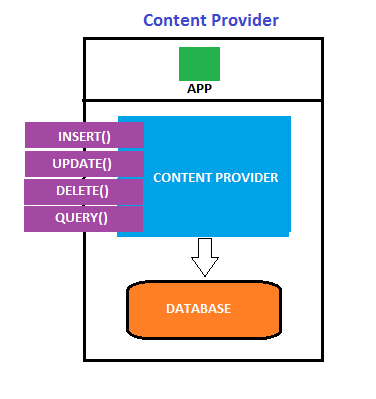
\includegraphics[scale=0.45]{android-provider.png}
\end{center}
\vspace{-20pt}
\caption{Provider}
\label{fig:android-provider}
\vspace{-30pt}
\end{wrapfigure}

Se encontró un provider {\color{blue}\texttt{``ar.sadosky.browser.history\_provider''}}, el cual tiene definida la propiedad \texttt{{\color{red}android:exported}={\color{blue}``true''}}, lo que significa que se exporta públicamente, y en donde la propiedad \texttt{\color{red}android:readPermission} no se encuentra definida. De esta forma, la aplicación está exponiendo \emph{datos sensibles} (el historial web del usuario), de forma pública, con \emph{permisos normales}, es decir que cualquier otra aplicación se encuentra en condiciones de leer el historial del usuario.

Para saber cómo una aplicación maliciosa podría aprovechar esta vulnerabilidad, es necesario entender cómo está definido el \emph{provider} dentro de la aplicación que se quiere vulnerar. Para ello, es útil primero entender qué es lo que viene a representar un \emph{content provider}, y cómo es que las aplicaciones acceden al mismo. En \fig{android-provider} se puede apreciar una representación básica de un provider en android, que no resulta ser más que una abstracción para una base de datos. 


\begin{figure}[H]
\lstinputlisting[language=XML_android]{AndroidManifest.xml}
\caption{AndroidManifest.xml}
\label{fig:AndroidManifest}
\end{figure}

\subsubsection{Prueba de Concepto}


\subsection{Componentes mal exportados}

%
%-- Sección: Vulnerabilidades de Red
%
\clearpage
\index{Vulnerabilidades de Red}
\section{Vulnerabilidades de Red}
\subsection{Activo}
\subsection{Pasivo}

%
%-- Sección: Vulnerabilidades Remotas
%
\clearpage
\index{Vulnerabilidades Remotas}
\section{Vulnerabilidades Remotas}


\end{document}